\chapter{How I Turned \(-\$20\) Million Into \(\$3.3\) Billion}

This chapter follows a School of Hard Knocks interview with Steven Klubeck, curated by LazyingArt LLC with Video2Book. There is no blackboard mathematics here, and no validated screenshot evidence carries equations or diagrams. The mathematical structure is commercial rather than physical: a negative starting point, a claimed multi-billion-dollar exit, a sequence of painful operating lessons, and a repeated mechanism in which trust becomes capital access, capital access supports scale, and scale becomes enterprise value.

\section{The Hook: From Millionaire Question to Billion-Dollar Exit}

The opening is built on a correction. The interviewer recalls stopping a man in Beverly Hills and asking the usual question: how old were you when you became a millionaire? Klubeck refuses the premise. The right category, he says, is billionaire.

Then the numbers come fast. The business was hospitality. He owned hotels. He says the company operated in \(35\) countries. Hilton, he says, owns the company today. The opening also preserves a useful ambiguity: the transcript places \(\$2.2\) billion, \(\$3.3\) billion equity value, and enterprise value very close together. We should not clean that into a more exact finance statement than the source gives us.

The safest quantitative coordinates are therefore these interview-backed claims:
\begin{align}
W_0 &\approx -\$20\,\text{million},\\
V_{\text{exit}} &\approx \$3.3\,\text{billion},\\
N_{\text{countries}} &= 35,\\
N_{\text{views}} &> 100\,\text{million}.
\end{align}
Here \(W_0\) is not an audited variable; it is the narrated starting point from the earlier viral clip. Likewise \(V_{\text{exit}}\) is a compact label for the value claim, not a resolved distinction between enterprise value and equity value.

The return visit changes the question. We are no longer only watching a street-interview surprise. We are asking how a broken position becomes a business that can be sold to Hilton. The interview does not begin that answer with valuation theory. It begins with a bad construction project.

\section{The Broken First Lesson}

Klubeck's first origin story is not Polo Towers. It is the shopping center before the hotel. He says he had never built a hotel; he had built shopping centers. One shopping center gave him nearly every problem imaginable: contractors went broke, he paid for lumber twice, he did not understand lien releases, tenants failed, the economy deteriorated, and an expensive retaining wall appeared outside the plans.

The result was not a clean win. He says he lost the shopping center, though he did not go broke. But the story's function is not to celebrate the loss. It is to explain why the next project was possible. A failed project forced construction literacy onto him: reading plans, understanding the jobsite, dealing with surprises, and surviving pressure without the comfort of theory.

In the notation of this chapter, the project is a capability update:
\begin{equation}
\text{failed project}
\;\longrightarrow\;
\text{construction literacy}
\;\longrightarrow\;
\text{hotel-building capability}.
\end{equation}

\subsection{Question \& Answer}

\paragraph{Question.}
How can losing the first project still become the asset?

\paragraph{Answer.}
Because the loss did not only remove value. It produced information. It exposed contractor risk, legal-release risk, tenant risk, cost-overrun risk, and plan risk all at once. If \(K_t\) is operating knowledge at stage \(t\), and \(L_t\) is the lesson extracted from a painful project, the update is
\begin{equation}
K_{t+1}=K_t+L_t.
\end{equation}
The danger is to write only
\begin{equation}
\text{project loss}=\text{failure}.
\end{equation}
The interview's actual logic is closer to
\begin{equation}
\text{project loss}
+
\text{survival}
+
\text{lesson extraction}
=
\text{future capability}.
\end{equation}

That is why this beat must not be compressed into generic adversity. The details matter because each failure mode becomes part of the operator's later range.

\section{Polo Towers: Customer Fit and Defensible Brand}

The next move is Polo Towers in Las Vegas. Klubeck says he was \(29\) years old, and that Polo Towers was the largest hotel-timeshare complex ever built at one time in the world. He says it was done on time and on budget, with his father involved because he was working for him at the time.

The interview immediately turns from construction to customer fit. The word ``polo'' could have made the project feel stiff, elite, or old-English. Klubeck says the customer was a broad market, so the project had to feel modern and comfortable rather than socially distant. The brand had to be aspirational without making the buyer feel unwelcome.

A compact reconstruction of that design rule is:
\begin{equation}
\text{useful brand}
=
\text{aspiration}
+
\text{customer comfort}
+
\text{defensibility}.
\end{equation}
The defensibility term matters because Klubeck says Ralph Lauren sued over the name. His account is that Polo Towers had been marked for hotel, timeshare, and casino uses, while Ralph Lauren had not done so in that domain. Whether one later verifies the legal record or not, the interview's point is clear: names, domains, and trademarks are not decoration. They are part of what the business owns or controls.

\begin{figure}
\centering
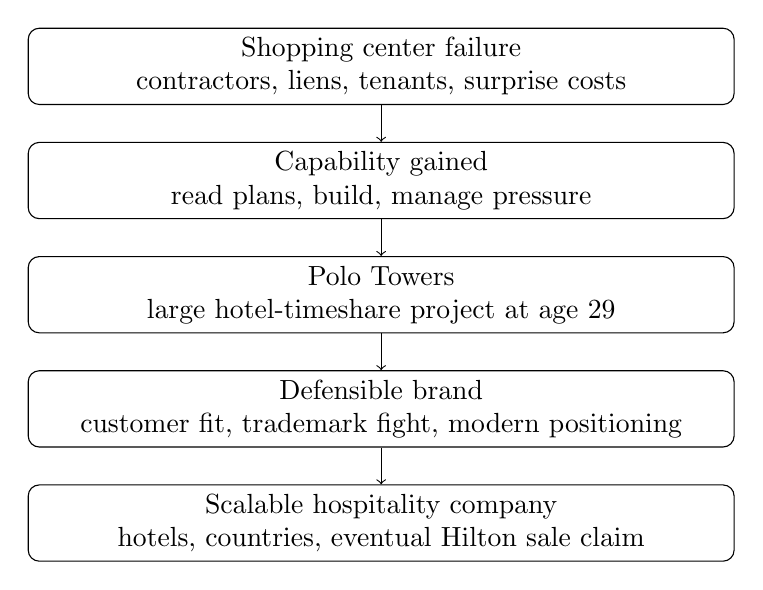
\begin{tikzpicture}[x=1cm,y=1cm]
\node[draw, rounded corners, align=center, text width=.72\linewidth] (a) at (0,0) {Shopping center failure\\contractors, liens, tenants, surprise costs};
\node[draw, rounded corners, align=center, text width=.72\linewidth] (b) at (0,-1.45) {Capability gained\\read plans, build, manage pressure};
\node[draw, rounded corners, align=center, text width=.72\linewidth] (c) at (0,-2.9) {Polo Towers\\large hotel-timeshare project at age \(29\)};
\node[draw, rounded corners, align=center, text width=.72\linewidth] (d) at (0,-4.35) {Defensible brand\\customer fit, trademark fight, modern positioning};
\node[draw, rounded corners, align=center, text width=.72\linewidth] (e) at (0,-5.8) {Scalable hospitality company\\hotels, countries, eventual Hilton sale claim};
\draw[->] (a) -- (b);
\draw[->] (b) -- (c);
\draw[->] (c) -- (d);
\draw[->] (d) -- (e);
\end{tikzpicture}
\caption{A transcript-grounded reconstruction of the path from a failed shopping-center project to a scalable hospitality company. No screenshot evidence is paired with this diagram because no validated frame contains a board diagram.}
\end{figure}

\section{Brand as a Trust Ledger}

Before the interview returns to detailed operations, Klubeck broadens the frame. He talks about helping create Brand USA, tourism and travel after what he calls the lost decade of travel, reporting to the Oval Office, and getting work done without trophies or red carpet. The institutional claims should remain source-conscious, but their role in the chapter is plain: the hotel story is being connected to a larger theory of brand, service, and public trust.

The brand section sharpens after the interviewer brings up superheroes as personal brands: figures that stand for and against something. Klubeck answers with integrity. A brand, he says in substance, takes decades to build and minutes to kill. If someone lies to a customer, trust is broken. If trust is broken, brand value is impaired.

Let \(B_t\) denote brand trust, \(S_t\) the service actually delivered, \(P_t\) the promise made, and \(D_t\) the damage from dishonesty or betrayal. A cautious ledger model is
\begin{equation}
B_{t+1}=B_t+\alpha(S_t-P_t)-D_t.
\end{equation}
This is not a measured empirical formula. It is a disciplined way to preserve the interview's mechanism. Good service can build trust incrementally, but a serious trust breach can subtract value quickly.

\subsection{Question \& Answer}

\paragraph{Question.}
Why fire the number-one salesperson if that person produces revenue?

\paragraph{Answer.}
Because the interview treats revenue and brand damage as different variables. A top salesperson may increase short-term sales, but if that person lies to customers, \(D_t\) becomes large. Klubeck says he fired the number-one salesperson because the person had become a cancer in the organization. He then claims the organization grew by about \(20\%\) after the removal:
\begin{equation}
\Delta_{\text{growth}}\approx 20\%
\quad
\text{after the firing, according to Klubeck.}
\end{equation}
This should be written as an anecdotal operating claim, not as causal proof. The important structure is the decision rule: brand is treated as a compounding asset, and dishonesty as a hidden liability.

\section{Operating Range: From Board Level to Making a Bed}

The interview then moves from brand principle to operating range. Klubeck says Marriott copied his company's Wall Street presentation deck. His CFO was upset; Klubeck read it as a compliment. But he says the large competitor could not replicate the company because his organization was nimble: a battleship that could move like a speedboat.

The explanation is not mystical. He says the chairman, CEO, and founder could talk about any job in the business. The transcript garbles one line about writing code, so we should state the safe point: he claims involvement across back-of-house software, tax, accounting, debits and credits, facilities management, and bed-making.

The scale claim is:
\begin{equation}
N_{\text{hotels}}>435,
\qquad
N_{\text{countries}}=35.
\end{equation}
What makes the claim instructive is the direction of the mechanism. Scale is not presented as escaping the details. It is presented as making details repeatable. Klubeck talks about towel placement, housekeeper videos, under-bed tent cards saying the company cleaned there too, cooking for guests, serving them, listening to them, and cleaning the table afterward.

A useful operating equation is therefore:
\begin{equation}
\text{scale}
=
\text{repeatable standards}
+
\text{local accountability}
+
\text{customer contact}.
\end{equation}
The founder's range matters because it turns standards from slogans into inspectable work. In this telling, no job is outside the leader's understanding, and that is how service becomes portable across properties.

\section{Crisis Finance and the Banks}

The central risk episode is 9/11. The transcript slows down here because the shock is concrete. There were no flights. Hotels had no guests. The cash registers went to zero. Before there is a lesson about transparency, there is the physical fact of demand disappearing.

The crisis chain is:
\begin{equation}
\text{flights grounded}
\rightarrow
\text{no guests}
\rightarrow
\text{zero cash registers}
\rightarrow
\text{bank communication}
\rightarrow
\text{additional borrowing}
\rightarrow
\text{survival}.
\end{equation}
Klubeck says he called his bank every day until the bank asked him to call every three days. He wanted lenders to know what was happening, and he says he had to borrow more money to get through it. The rule extracted from the episode is the same rule that appears in the brand section: tell the good, the bad, and the ugly.

\subsection{Question \& Answer}

\paragraph{Question.}
What keeps financing alive when revenue stops?

\paragraph{Answer.}
Not optimism by itself. The interview's answer is credibility. Klubeck says the banks saw capacity, character, and credit, the three C's of banking. In a crisis, the operator cannot honestly say that conditions are good. What he can do is reduce uncertainty for the lender by communicating early, candidly, and repeatedly.

\begin{table}
\centering
\begin{tabular}{p{.23\linewidth}p{.32\linewidth}p{.34\linewidth}}
\hline
Criterion & Meaning in the interview & Behavior shown \\
\hline
Capacity & Ability to perform or repay & Prior execution, repayment, and survival under pressure \\
Character & Trustworthiness under stress & Candid bank calls during the 9/11 demand shock \\
Credit & Lender confidence and financial record & Banks seeing him as good for the money \\
\hline
\end{tabular}
\caption{The three C's of banking as Klubeck uses them in the interview.}
\end{table}

The working principle is path dependence. If lenders and investors do well with an operator in one round, they are more likely to return in the next. Klubeck states the philosophy plainly: do not try to get the edge on somebody; make sure everyone does well together.

\section{Negotiation, Silence, and the Close}

After the bank discussion, the rhythm changes. The interviewer recalls Klubeck's rule that the first person who talks loses. Klubeck gives a case: he once waited a week after putting a deal in front of the other side. He wanted to pick up the phone. He did not. Eventually the call came.

The rule is simple enough to write as an algorithm:
\begin{enumerate}
\item Make the ask.
\item Put the decision in front of the other side.
\item Stop talking.
\item Resist the urge to repair silence with nervous speech.
\item After the sale is made, do not talk past the close.
\end{enumerate}

The anecdotal waiting time is
\begin{equation}
T_{\text{wait}}\approx 1\,\text{week}.
\end{equation}
But the mechanism is not that every negotiation requires one week. The mechanism is that excess speech after the ask can become a concession, an apology, or confusion. Silence is not empty space. In this passage, it is part of the structure of the close.

\section{After the Exit: California as the Next Broken Business}

The final pivot begins with a contrast. After selling a company for several billion dollars, Klubeck could have chosen leisure. Instead, he says he is running for governor of California. The explanation starts personally: he wanted to live his Beverly Hills dream after growing up in the San Fernando Valley. Then it becomes operational.

He says he interviewed candidates, studied his home state, and concluded that California is not merely a state but a country, calling it the fifth largest GDP in the world. Unless verified elsewhere, that remains an interview claim. He says California is on defense when it should be on offense. He says leaders did not talk to the state's best customers, and that customers fled.

The business diagnostic pattern returns:
\begin{align}
N_{\text{interviews}} &> 300,\\
\text{diagnosis} &= \{\text{not affordable},\ \text{not livable},\ \text{not workable}\},\\
\text{repair rule} &= \{\text{respect},\ \text{responsibility},\ \text{results}\}.
\end{align}
The politics should not be flattened into neutral fact, but the narrative structure is important. He is applying the same operator's sequence at a larger scale: identify the customer, listen to the customer, locate the broken process, and claim a mandate to repair it.

This completes the arc. A broken shopping center teaches capability. A broken brand rule teaches discipline. A broken travel market tests banking trust. A broken state becomes, in Klubeck's framing, the next operating problem.

\section{Summary}

The lecture unfolds as a chain of source-conscious operating claims. The first loss teaches construction. Polo Towers turns construction literacy into a branded asset. Brand becomes a trust ledger. A top salesperson can become a liability if trust is broken. Scale comes from repeatable standards, not distance from details. A demand shock like 9/11 tests whether banks trust the operator. Negotiation requires silence after the ask. Public service is then framed as the same repair problem at a larger scale.

The cleanest mathematical summary is not a wealth formula. It is a mechanism:
\begin{equation}
\text{painful evidence}
\rightarrow
\text{operating discipline}
\rightarrow
\text{trust}
\rightarrow
\text{capital access}
\rightarrow
\text{scale}
\rightarrow
\text{durable value}.
\end{equation}
The numbers give the story scale: \(-\$20\) million, \(\$3.3\) billion, \(35\) countries, more than \(435\) hotels, more than \(100\) million views. But the interview's repeated lesson is about what can make such numbers possible in Klubeck's account: learn under pressure, protect trust, stay close to the customer, and treat reputation as part of enterprise value.